% Copyright (c) 2026 CorrectBrain
% SPDX-License-Identifier: MIT

\PassOptionsToPackage{dvipsnames,svgnames,x11names}{xcolor}
\documentclass[tikz,border=8pt]{standalone}
\usetikzlibrary{arrows.meta,positioning,calc,shapes,shadows,decorations.pathmorphing,shapes.geometric,backgrounds,decorations.markings,decorations.pathreplacing,decorations.text,fit,shapes.misc,shapes.arrows,matrix,bending,3d,chains,intersections,shapes.symbols,svg.path,shapes.multipart,snakes,shapes.callouts,angles,quotes}
\providecolor{gold}{RGB}{212,175,55}
\providecolor{silver}{RGB}{192,192,192}
\providecolor{bronze}{RGB}{205,127,50}
\providecolor{darkblue}{RGB}{0,0,139}
\providecolor{lightblue}{RGB}{173,216,230}
\providecolor{darkgreen}{RGB}{0,100,0}
\providecolor{lightgreen}{RGB}{144,238,144}
\providecolor{darkred}{RGB}{139,0,0}
\providecolor{navy}{RGB}{0,0,128}
\providecolor{skyblue}{RGB}{135,206,235}
\providecolor{beige}{RGB}{245,245,220}
\providecolor{cream}{RGB}{255,253,208}
\usepackage{amsmath}
\usepackage{amssymb}
\usepackage{fontawesome5}
\usetikzlibrary{fadings,shadows.blur,patterns,patterns.meta}


\usepackage{amsmath}
\usepackage{amssymb}
\usepackage{fontawesome5}
\usepackage{xcolor}

\providecolor{gold}{RGB}{212,175,55}
\providecolor{silver}{RGB}{192,192,192}
\providecolor{bronze}{RGB}{205,127,50}
\providecolor{darkblue}{RGB}{0,0,139}
\providecolor{lightblue}{RGB}{173,216,230}
\providecolor{darkgreen}{RGB}{0,100,0}
\providecolor{lightgreen}{RGB}{144,238,144}
\providecolor{darkred}{RGB}{139,0,0}
\providecolor{navy}{RGB}{0,0,128}
\providecolor{skyblue}{RGB}{135,206,235}
\providecolor{beige}{RGB}{245,245,220}
\providecolor{cream}{RGB}{255,253,208}

% --- COLOR PALETTE (LIGHT THEME / BLUEPRINT AESTHETIC) ---
\definecolor{canvasbg}{RGB}{255, 255, 255}
\definecolor{deepslate}{RGB}{26, 43, 60}
\definecolor{steelblue}{RGB}{43, 91, 132}
\definecolor{panelbg}{RGB}{255, 255, 255}
\definecolor{panelborder}{RGB}{220, 226, 235}
\definecolor{containerbg}{RGB}{248, 249, 250}
\definecolor{containerborder}{RGB}{180, 190, 205}
\definecolor{paddinggold}{RGB}{243, 156, 18}
\definecolor{idebg}{RGB}{40, 44, 52}
\definecolor{codekw}{RGB}{224, 108, 117}
\definecolor{codenum}{RGB}{152, 195, 121}
\definecolor{codecomment}{RGB}{127, 132, 142}
\definecolor{codeaccent}{RGB}{97, 175, 239}
\definecolor{accentpink}{RGB}{214, 51, 108}
\definecolor{accentblue}{RGB}{13, 110, 253}
\definecolor{accentorange}{RGB}{217, 119, 6}
\definecolor{measureblue}{RGB}{30, 90, 180}
\definecolor{measureorange}{RGB}{210, 100, 15}
\definecolor{measurenavy}{RGB}{26, 43, 60}

\begin{document}
\begin{tikzpicture}[
    panel/.style={
        fill=panelbg,
        draw=panelborder,
        line width=1pt,
        rounded corners=10pt,
        blur shadow={shadow opacity=20, shadow blur steps=6, shadow blur radius=4pt, shadow xshift=1.5pt, shadow yshift=-2.5pt}
    },
    measure/.style={Latex-Latex, thick},
    pointer/.style={-Stealth, line width=2.5pt}
]

% Background block enforcing pure white canvas
\fill[canvasbg] (0.0, -3.0) rectangle (34.0, 21.0);

% =========================================================================
% 1. TYPOGRAPHY & TITLES (Strict Coordinates)
% =========================================================================
\node[font=\Huge\bfseries\color{deepslate}, align=center] at (16.9633,20.1242) {The Geometry of the Padding-Bottom Hack};
\node[font=\Large\color{steelblue}, align=center] at (17,19.2062) {Exploiting CSS Specifications for Intrinsic Aspect Ratios};

% =========================================================================
% 2. LEFT PANELS (Text & Math with Zero Overlap)
% =========================================================================

% --- CSS BOX MODEL SPEC PANEL (Anchor north west at (0.5, 18.0), text width=8.5cm, inner sep=14pt) ---
\node[panel, text width=8.5cm, inner sep=14pt, anchor=north west] (spec) at (0.5, 18.0) {
    \textbf{\Large\color{accentpink}\faBook \ CSS Box Model Spec}\\[8pt]
    \color{deepslate}\large
    Why does \texttt{padding-bottom} create height relative to width? \\[6pt]
    Because the W3C CSS Spec explicitly states:
    \begin{quote}
    \itshape\color{accentorange}"The percentage is calculated with respect to the \textbf{width} of the generated box's containing block..."
    \end{quote}
    \vspace{2pt}
    This quirk applies to \textbf{both} padding-top and padding-bottom!
};

% --- THE 16:9 MATH PANEL (Anchor north west at (0.5, 10.0), text width=8.5cm, inner sep=14pt) ---
\node[panel, text width=8.5cm, inner sep=14pt, anchor=north west] (math) at (0.5, 10.0) {
    \textbf{\Large\color{steelblue}\faCalculator \ The 16:9 Math}\\[6pt]
    \color{deepslate}\large
    We need an empty box where the Height is exactly proportional to the Width.
    \vspace{6pt}
    $$ \text{Ratio} = \frac{\text{Height}}{\text{Width}} $$
    \vspace{6pt}
    $$ 16:9 \rightarrow \frac{9}{16} = \mathbf{0.5625} $$
    \vspace{6pt}
    Expressed as a percentage of the width:
    \vspace{6pt}
    $$ \color{accentblue}\mathbf{0.5625 \times 100\% = 56.25\%} $$
};

% =========================================================================
% 3. THE GRAPHIC AREA (Right Side: DOM Inspector / Viewport Aesthetic)
% =========================================================================

% --- CONTAINING BLOCK (X: 11.0 to 28.0, Y: -0.5 to 16.5) ---
\draw[draw=containerborder, line width=1.5pt, rounded corners=8pt, fill=containerbg, drop shadow={shadow opacity=15, shadow blur steps=4, shadow xshift=2pt, shadow yshift=-3pt}] (11.0, -0.5) rectangle (28.0, 16.5);

% Browser Window Chrome / Header (Y: 15.5 to 16.5)
\fill[panelborder!60, rounded corners=8pt] (11.0, 15.5) rectangle (28.0, 16.5);
\fill[containerbg] (11.0, 15.5) rectangle (28.0, 15.7);
\draw[draw=containerborder, line width=1pt] (11.0, 15.5) -- (28.0, 15.5);

% Window Action Dots
\fill[red!75!black] (11.4, 16.0) circle (3pt);
\fill[orange!85!black] (11.7, 16.0) circle (3pt);
\fill[green!75!black] (12.0, 16.0) circle (3pt);

% Containing Block Label
\node[font=\bfseries\color{deepslate}, anchor=west] at (12.4, 16.0) {\faBoxOpen \ Containing Block (\texttt{width: 100\%})};

% Container Width Measurement Arrow (Y: -1.5)
\draw[measure, color=measurenavy, line width=1.5pt] (11.0, -1.5) -- (28.0, -1.5) node[midway, below=6pt, font=\large\bfseries] {$W_{\text{container}}$ (e.g., 1000px)};

% --- THE ASPECT RATIO BOX (16 units wide x 9 units tall -> 16:9) ---
% Position: (11.5, 6.0) to (27.5, 15.0)

% 1. Padding Area Fill (Translucent Gold)
\fill[paddinggold!20, rounded corners=3pt] (11.5, 6.0) rectangle (27.5, 15.0);

% 2. 16:9 Internal Coordinate Proof Grid (16 cols x 9 rows, step = 1.0)
\draw[step=1.0, color=orange!45, line width=0.55pt] (11.5, 6.0) grid (27.5, 15.0);

% 3. Aspect Ratio Box Outline
\draw[draw=paddinggold!85!black, dashed, line width=1.5pt, rounded corners=3pt] (11.5, 6.0) rectangle (27.5, 15.0);

% 4. Content Line (height: 0) represented by a thick red line flush with Chrome bottom (Y = 15.0)
\draw[red!85!black, line width=3.5pt] (11.5, 15.0) -- (27.5, 15.0);

% Badges for Content Line & Padding Box (Zero Overlap, Strict Bounding)
\node[fill=red!85!black, text=white, font=\scriptsize\bfseries, rounded corners=2pt, inner sep=4pt, fill opacity=1, text opacity=1, anchor=south west] at (11.5, 15.1) {\faLayerGroup \ Content Box (\texttt{height: 0})};
\node[fill=paddinggold!90!black, text=white, font=\scriptsize\bfseries, rounded corners=2pt, inner sep=4pt, fill opacity=1, text opacity=1, anchor=north east] at (27.5, 5.6) {\faLayerGroup \ \texttt{.aspect-ratio-box} (Generated by \texttt{padding-bottom})};

% 5. CSS IDE Code Window (Relocated to dedicated void: center-anchored at (19.5, 3.25))
\node[fill=idebg, rounded corners=6pt, inner sep=10pt, drop shadow={shadow opacity=30, shadow blur steps=4, shadow xshift=2pt, shadow yshift=-2.5pt}, align=left, anchor=center] at (18.7107,2.9012) {
    \fontsize{10}{14.5}\selectfont\ttfamily
    \color{white}\textbf{.aspect-ratio-box} \{\\
    \quad \color{codekw}width\color{white}: \color{codenum}100\%\color{white};\\
    \quad \color{codecomment}/* height is 0, all vertical space */\\
    \quad \color{codecomment}/* comes from padding-bottom */\\
    \quad \color{codekw}height\color{white}: \color{codenum}0\color{white};\\
    \quad \color{codekw}padding-bottom\color{white}: \color{codeaccent}\textbf{56.25\%}\color{white};\\
    \color{white}\}
};

% Measurements on the wrapper and padding
\draw[measure, color=measureblue, line width=1.5pt] (11.5, 17.5) -- (27.5, 17.5) node[midway, above=8pt, font=\small\bfseries] {Wrapper Width = $100\%$ of $W_{\text{container}}$ (16 units)};
\draw[measure, color=measureorange, line width=1.5pt] (28.5, 6.0) -- (28.5, 15.0) node[midway, right=8pt, align=left, font=\small\bfseries] {\textbf{Padding Bottom}\\$= \mathbf{56.25\%} \times W_{\text{container}}$\\$= \frac{9}{16} \times W_{\text{container}}$ (9 units)\\$= 562.5\text{px}$};

% =========================================================================
% 4. CONNECTOR ROUTING (POINTERS ACROSS GUTTER)
% =========================================================================

% Pointer 1: CSS Spec Panel to Content Line (height: 0)
\draw[pointer, color=red!85!black] (10.0, 15.0) -- (11.5, 15.0);

% Pointer 2: Math Panel to Padding Area Grid
\draw[pointer, color=steelblue] (10.0, 9.5) -- (11.5, 9.5);

\end{tikzpicture}
\end{document}
